\section{溶液物性および圧力場の確認}
\subsection{粘度 計測結果}
球落下実験を行う試験溶液として,異なる質量濃度のPAA溶液を製作した.この製作した溶液の粘度特性を,粘度計を用いて計測した.なお,溶媒中の溶質が不均一な状態や,混合時に混入する気泡が存在する状態では,溶液の粘度が正しく計測できない.十分な溶質拡散や脱泡には時間を要するため,粘度計測は溶液作製直後ではなく,1週間後に行った.それぞれの試料に対し,円錐回転子の回転数を変化させることでせん断速度を変化させ,粘度を各5回計測し,その平均を求めた.

水道水の粘度計測結果をFig.\ref{fig:vis}(a)に示す.なお,縦軸は粘度,横軸はせん断速度を表す.2.3節で示されたように,コーンロータの回転速度に応じて,液体のせん断速度を変化させた.その結果,粘度は1.1mPa$\cdot$sでほぼ一定となった.これは,水がニュートン流体であり,速度勾配とせん断応力が比例することを表す.理科年表\cite{理科年表}によると,水道水の粘度は20℃で1.0mPa$\cdot$sとなっており,適切に粘度計測が行われていたと考えられる.

PAA溶液の粘度計測結果をFig.\ref{fig:vis}(b)に示す.なお,縦軸は粘度の対数,横軸はせん断速度の対数を表す.溶液の濃度が上昇すると,粘度が大きくなった.ここで,Power-law modelに従うものとすると,せん断速度$\dot{\gamma}$より粘度$\mu$は次式で表される\cite{ref:1}.
\begin{eqnarray}
	\label{eq:power-low}
	\mu=k\cdot\dot{\gamma}^{n-1} .
\end{eqnarray}
ここで,$k$は粘度定数,$n$は粘度指数である.式(\ref{eq:power-low})で計測値をフィッティングした線の$k,n$の値を,Table \ref{table:power-law}に示す.溶液の濃度が濃いほど,$n$は小さくなる.これは擬塑性が強くなることを表す.

\begin{figure}[ht]
	\centering
	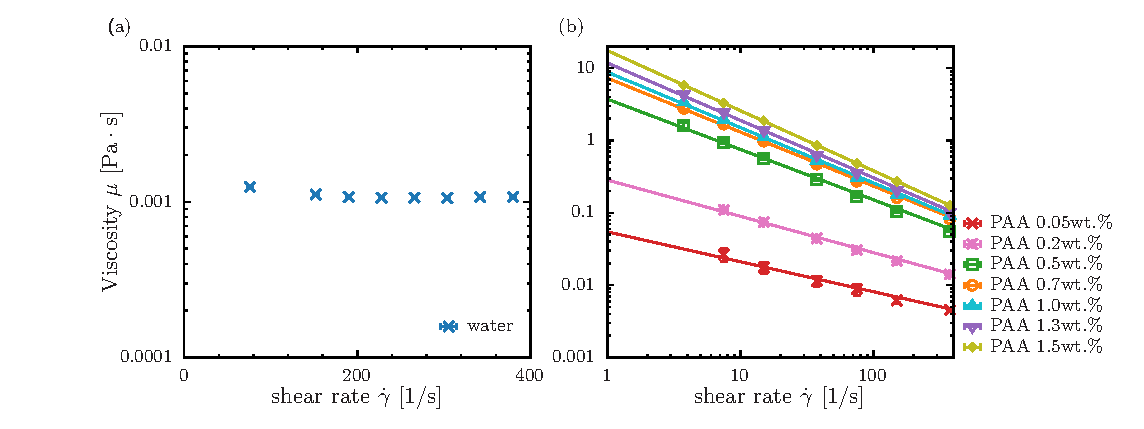
\includegraphics[width=1\textwidth]{3-Physical_Property/viscosity.eps}
	\caption{Viscosity versus shear rate for (a) tap water, (b) PAA solution.}
	\label{fig:vis}
\end{figure}

\begin{table}[h]
	\centering
	\caption{Parameters $k$ and $n$ in the Power-law model for each PAA solution at each concentration.}
	\label{table:power-law}
	\begin{tabular}{c|c|c|c|c|c|c|c} \hline
		PAA[wt.\%] & 0.05  & 0.2  & 0.5  & 0.7  & 1.0  & 1.3  & 1.5  \\ \hline \hline
		$k$        & 0.054 & 0.28 & 3.7  & 7.3  & 8.8  & 12   & 18   \\ \hline
		$n$        & 0.59  & 0.50 & 0.30 & 0.25 & 0.23 & 0.21 & 0.17 \\ \hline
	\end{tabular}
\end{table}

\newpage

\subsection{弾性率 計測結果}
\label{sec:elasticity}

作製したPAA溶液の弾性特性を得るため,それぞれのPAA質量濃度における,貯蔵弾性率$G'$,損失弾性率$G''$の応力依存性を計測した.また,式(\ref{eq:loss_factor})より損失正接$\tan\left(\eta\right)$を求めた.計測結果をFig.\ref{fig:PAA-elast}に示す.印可する応力が小さい場合,損失正接が1より小さく弾性による影響が強かった.また,応力を大きくすると,損失正接が1より大きくなり粘性による影響が強くなった.これより,応力が小さい場合は弾性による影響が,大きい場合は粘性による影響が大きくなることが分かった.加えて,濃度が濃くなると,貯蔵弾性率,損失弾性率共に大きくなった.これより濃度が高くなると溶液の粘弾性が強くなることが分かった.

ここで,損失正接が1となる応力$\tau$を$\tau_0$と定義する.各質量濃度における,$\tau_0$を内挿によって求めた結果をTable.\ref{table:PAA-tau0}に示す.質量濃度が上昇すると,$\tau_0$が大きくなった.このことより,濃度の増加に伴い,弾性による影響が大きくなる事が分かった.

\begin{figure}[ht]
	\centering
	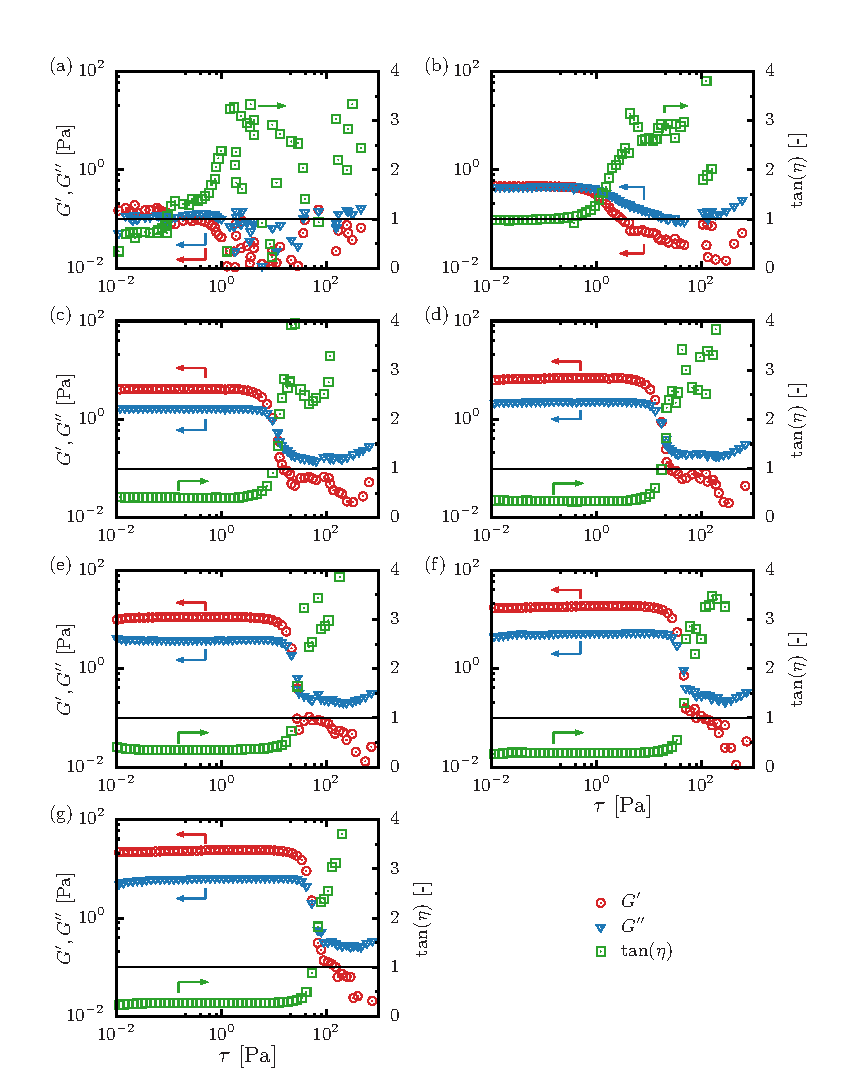
\includegraphics[width=1\textwidth]{3-Physical_Property/elastic_modulus.eps}
	\caption{Stress dependence of storage and loss elastic moduli for (a)0.05wt.\% (b)0.2wt.\% (c)0.5wt.\% (d)0.7wt.\% (e)1.0wt.\% (f)1.3wt.\% (g)1.5wt.\%.}
	\label{fig:PAA-elast}
\end{figure}

\begin{table}[h]
	\centering
	\caption{Relationship between concentration and $\tau_0$ for PAA solution.}
	\label{table:PAA-tau0}
	\begin{tabular}{c|c|c|c|c|c|c|c} \hline
		PAA[wt.\%]   & 0.05  & 0.2  & 0.5 & 0.7 & 1.0 & 1.3 & 1.5 \\ \hline \hline
		$\tau_0$[Pa] & 0.082 & 0.11 & 9.9 & 18  & 22  & 40  & 55  \\ \hline
	\end{tabular}
\end{table}

\clearpage

\subsection{圧力振幅 計測結果}

それぞれの質量濃度において,超音波圧力振幅の計測を行った.結果をFig.\ref{fig:pressure}に示す.縦軸は水槽液面からの深さ,横軸は圧力振幅である.図より,容器内に形成する圧力場は,周期的な振幅で分布する.これは定在波の性質を示し,共振状態にあることで,圧力振幅が数気圧分に至る.この結果より,圧力振幅$\Delta{}P$の$y$方向平均値$\Delta\overline{P}$をTable \ref{table:press}に示す.

\begin{table}[h]
	\centering
	\caption{Averaged value of pressure amplitude.}
	\label{table:press}
	\begin{tabular}{c|c|c|c|c|c|c|c} \hline
		PAA[wt.\%]                & 0.05  & 0.2   & 0.5   & 0.7   & 1.0   & 1.3   & 1.5   \\ \hline \hline
		$\Delta\overline{P}$[kPa] & 112.2 & 129.7 & 143.8 & 150.3 & 156.2 & 199.5 & 191.1 \\ \hline
	\end{tabular}
\end{table}

\begin{figure}[ht]
	\centering
	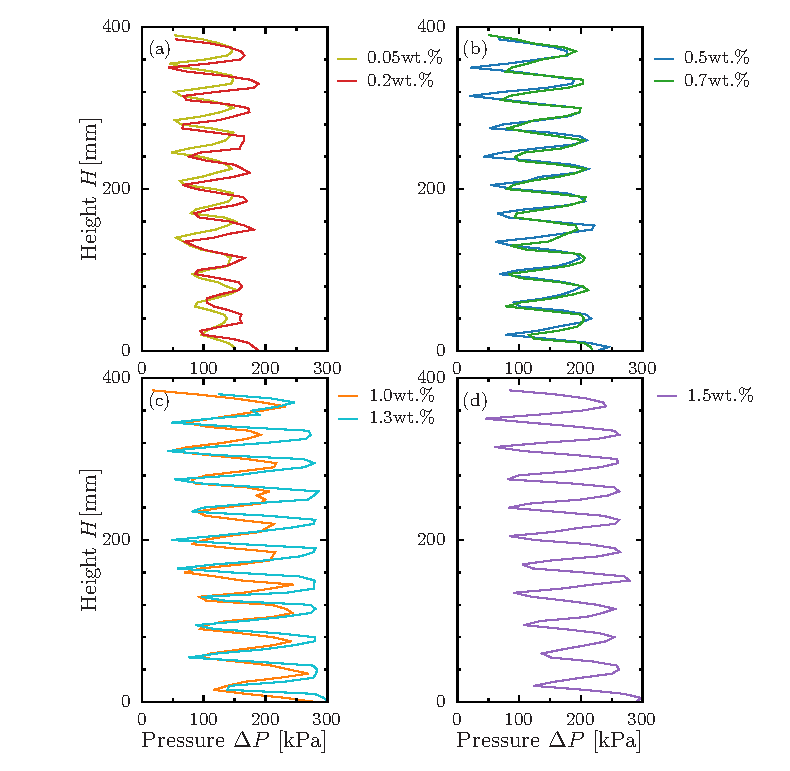
\includegraphics[width=0.9\textwidth]{3-Physical_Property/press.eps}
	\caption{Average pressure amplitude in (a)0.05wt.\% amd 0.2wt.\%, (b)0.5wt.\% and 0.7wt.\%, (c)1.0wt.\% and 1.3wt.\%, (d)1.5wt.\% PAA solution.}
	\label{fig:pressure}
\end{figure}
